% De la numérisation à l’annotation

\subsection{\textit{Workflow} d'annotation}
    \subsubsection{Sous-sous-section 1}
 La chaîne de traitement proposée par \eida (fig. \ref{fig:eida_workflow}) propose ainsi une alternance d'étapes automatisées, en bleu sur le schéma, et d'étapes d'analyse par les chercheurs du projet.

\begin{figure}[h]
	\centering
	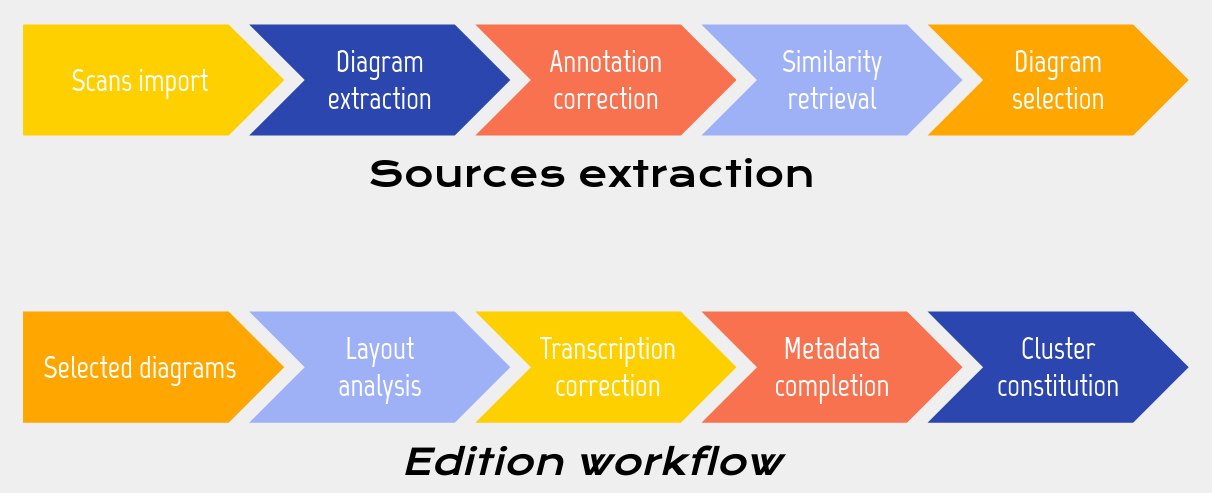
\includegraphics[width=15cm]{images/eida_workflow.png}
	\caption{\textit{Workflow} de traitement des sources du projet \eida}
	\label{fig:eida_workflow}
\end{figure}

    \subsubsection{Sous-sous-section 2}

    
    \subsection{Échanges et transformation des données}
        \subsubsection{Sous-sous-section 1}


        \subsubsection{Sous-sous-section 2}


    \subsection{Interface d’annotation}
        \subsubsection{Sous-sous-section 1}


        \subsubsection{Sous-sous-section 2}

